\documentclass[a4paper]{article}
\usepackage[english]{babel}
\usepackage[utf8x]{inputenc}
\usepackage{graphicx}
\usepackage{caption}
\usepackage{pmboxdraw}
\usepackage{color}
\usepackage{tocloft}
\definecolor{darkgray}{rgb}{0.41, 0.41, 0.41}
\definecolor{green}{rgb}{0.0, 0.5, 0.0}

\usepackage{listingsutf8}
\lstset{language=Java, 
	numbers=left,
	stepnumber=5,
	firstnumber=1,
	numberfirstline=true,
    basicstyle=\linespread{0.8}\ttfamily,
    keywordstyle=\color{blue}\ttfamily,
	showstringspaces=false,
    stringstyle=\color{red}\ttfamily,
    commentstyle=\color{green}\ttfamily,
	identifierstyle=\color{darkgray}\ttfamily,
	tabsize=1,
    breaklines=true,
    extendedchars=true,
	inputencoding=utf8x,
    escapeinside={\%*}{*)},
}


\setlength{\tabcolsep}{6pt}
\setlength\cftaftertoctitleskip{20pt}
\begin{document}
\setlength{\textwidth}{16cm}
\setlength{\textheight}{22cm}


\title{
\includegraphics[scale=0.15]{resources/img/feup_logo.png}
\linebreak\linebreak\linebreak\linebreak\linebreak
\Huge\textbf{Formal Modeling of a Tetris Game }\linebreak\linebreak
\linebreak\linebreak
\Large{Mestrado Integrado em Engenharia Informática e Computação} \linebreak\linebreak
\Large{Métodos Formais em Engenharia de Software}\linebreak\linebreak
}
\author{\textbf{Grupo 1 Turma 4MIEIC02}\\
Ângela Cardoso - up200204375\\
Tiago Galvão - up201500034\\
Nuno Valente - up200204376\\
\linebreak\linebreak \\
\linebreak\linebreak\linebreak
\linebreak\linebreak\vspace{1cm}}

\maketitle

\thispagestyle{empty}
\newpage
\tableofcontents
\newpage

\section{Informal system description and list of requirements}

\subsection{Informal system description}
\label{informal-rules}

\paragraph{ }Tetris game it's a puzzle game and one of the most recognizable and influential video game brands in the world. It’s no wonder why there are hundreds of millions of Tetris products being played, worn, and enjoyed by fans in their everyday lives. The game was born in 1984 and it's living proof of a game that have truly transcended the barriers of culture and language.

\paragraph{ }A meritorious reference to Alexey Pajitnov because he his the person who developed this popular game. He is a russian video game designer and computer engineer and in his spare time, he drew inspiration from his favorite puzzle board game, pentominoes, and decided to create a computer game for himself. Pajitnov envisioned an electronic game that let players arrange puzzle pieces in real time as they fell from the top of the playing field. The resulting design was a game that used seven distinctive geometric playing pieces (appendix\ref{tetrominoes}), each made up of four squares. Pajitnov called this game “Tetris,” a combination of “tetra” (the Greek word meaning “four”) and “tennis” (his favorite sport).

\paragraph{ }The rules to play the game are very simple. Tetris game requires players to strategically rotate and drop a chaining of tetrominoes that fall into the rectangular board at increasing speeds. Players attempt to clear as many lines as possible by completing horizontal rows of blocks without empty space, but if the tetrominoes surpass the skyline(top of the board) the game is over! Speed and consequent level advance can make the game ally to strategy more enthusiastic. Formal details about other rules are presented in appendix\ref{rules}.

\textcolor{red}{put a game image here}
\subsection{List of requirements}
\label{sec:requirements}
\begin{table}[h]
	\centering
	%\caption{My caption}
	\label{tab:list-of-requirements}
	\begin{tabular}{|l|l|p{9cm}|}
		\hline
		\textbf{Id} & \textbf{Priority} & \textbf{Description} \\ \hline
		R1 & Mandatory         & The player can view his score and level \\ \hline
		R2 & Mandatory         & The game allows two movements - rotation and drop \\ \hline
		R3 & Opcional         & The player should be able to leave the game when he wants \\ \hline
		R4 & Mandatory         & The player has access to a footnote where are the rules to play the game \\ \hline
		R5 & Mandatory         & The spawns appears in a random order to be played\\ \hline
		R6 & Mandatory         & When a row(s) is(are) full of blocks it(they) must be cleared \\ \hline
		R7 & Mandatory         & If tetraminoes surpass the skyline the game is over \\ \hline
		R8 & Opcional          & Time to time the level advance one degree and the game became more difficult \\ \hline
		R9 & Mandatory        & Each tetromino is formed by four squares named minos by us \\ \hline
		R10 & Mandatory        & The player has access to his score and actual level where he is \\ \hline
	\end{tabular}
\end{table}

These requirements are directly translated onto use cases as shown next.
\section{Visual UML model} 


\subsection{Use case model}

In all use cases we've made an assumption that all keyboard game keys are functioning properly.

\begin{center}
	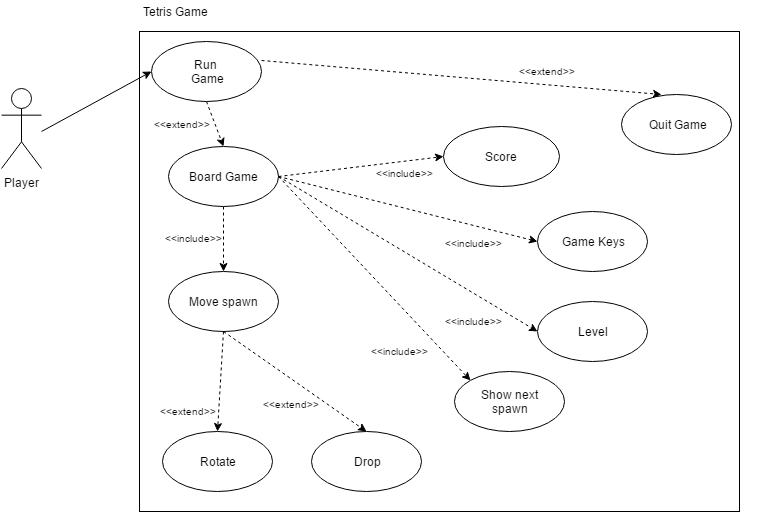
\includegraphics[scale=0.47]{resources/img/use_cases}
	\label{use-cases}
\end{center}

The main use cases are described below: 

\begin{table}[h]
	\centering
	%	\caption{Use case configuration}
	\label{use-case-configuration}
	\begin{tabular}{|l| p{9cm}|}
		\hline
		\textbf{Scenario}        & \textbf{Configure Game} \\ \hline
		\textbf{Description}     &  The user can write his nickname and difficulty level\\ \hline
		\textbf{Pre-conditions}  & 	
		\begin{tabular}[c]{@{}l@{}}
			The game is in the configuration menu
		\end{tabular}  \\ \hline
		\textbf{Post-conditions} &  The player became associated with that nickname and game with difficulty level \\ \hline
		\textbf{Steps}           &  (none) \\ \hline
		\textbf{Exceptions}      &  (none) \\ \hline
	\end{tabular}
\end{table}

\begin{table}[h]
	\centering
%	\caption{Use case rotation}
	\label{use-case-rotation}
	\begin{tabular}{|l| p{9cm}|}
		\hline
		\textbf{Scenario}        & \textbf{Rotation Movement} \\ \hline
		\textbf{Description}     &  Rotate a tetromino when is falling \\ \hline
		\textbf{Pre-conditions}  & 	
			\begin{tabular}[c]{@{}l@{}}
				 Tetromino must not be frozen in place
			 \end{tabular}  \\ \hline
		\textbf{Post-conditions} &  Tetromino position has changed  \\ \hline
		\textbf{Steps}           &  The player must click on a key that allows rotation  \\ \hline
		\textbf{Exceptions}      &  Tetromino type O doesn't have other form when try rotation; when, simultaneously, try to rotate and the spawn reached one final position; the stack of tetrominoes reached the penult line of the board \\ \hline
	\end{tabular}
\end{table}

\begin{table}[h]
	\centering
	%	\caption{Use case drop}
	\label{use-case-drop}
	\begin{tabular}{|l| p{9cm}|}
		\hline
		\textbf{Scenario}        & \textbf{Drop Movement} \\ \hline
		\textbf{Description}     &  Accelerates the tetromino falling and position it as it was before reach the final position \\ \hline
		\textbf{Pre-conditions}  & 	
		\begin{tabular}[c]{@{}l@{}}
			Tetromino must not be frozen in place
		\end{tabular}  \\ \hline
		\textbf{Post-conditions} &  Tetromino position has changed  \\ \hline
		\textbf{Steps}           &  The player must click on a key that allows falling spawn  \\ \hline
		\textbf{Exceptions}      &  (none) \\ \hline
	\end{tabular}
\end{table}

\subsection{Class model}

\begin{center}
	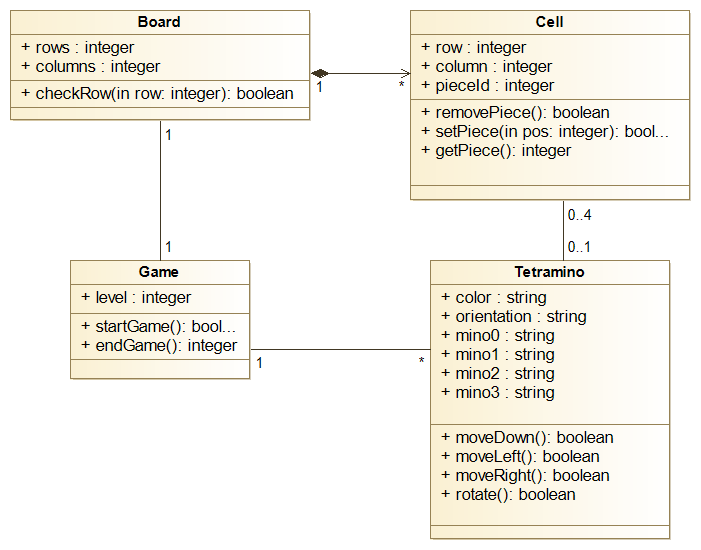
\includegraphics[scale=0.4]{resources/img/uml}
	\label{uml}
\end{center}

\begin{table}[!h]
	\centering
	\label{description-classes}
	\begin{tabular}{|l|p{10cm}|}
	\hline
	\textbf{Class} 			   & \textbf{Description}	\\	\hline
	Game		   			   &	Core model; defines the state variables and operations available to the players	\\	\hline
	Board		   			   &	Defines a game environment for playing and where eachhpiece of tetraminoes can stay \\	\hline
	Tetromino	   			   &	Defines one general piece to play with	\\	\hline
	TetrominoI/J/L/O/S/T/Z	   &	Defines one specific piece and is a subclass of Tetromino \\	\hline
	TestCaseExtra  			   &	Superclass for test classes; defines assertEquals and assertTrue	\\	\hline
	TestTetris	   			   &	Defines the test/usage scenarios and test cases for the tetris game	\\	\hline
	\end{tabular}
	\caption{Description of each class}
\end{table}

\section{Formal VDM++ model}

\subsection{Class Game}

\lstinputlisting{../tetris.vdm/Game.vdmpp}

\subsection{Class Board}

%\lstinputlisting{../tetris.vdm/Board.vdmpp}

\subsection{Class Tetromino}

\lstinputlisting{../tetris.vdm/Tetramino.vdmpp}

\subsubsection{Class TetrominoI}

\lstinputlisting{../tetris.vdm/TetraminoI.vdmpp}

\subsubsection{Class TetrominoJ}

\lstinputlisting{../tetris.vdm/TetraminoJ.vdmpp}

\subsubsection{Class TetrominoL}

\lstinputlisting{../tetris.vdm/TetraminoL.vdmpp}

\subsubsection{Class TetrominoO}

\lstinputlisting{../tetris.vdm/TetraminoO.vdmpp}

\subsubsection{Class TetrominoS}

\lstinputlisting{../tetris.vdm/TetraminoS.vdmpp}

\subsubsection{Class TetrominoT}

\lstinputlisting{../tetris.vdm/TetraminoT.vdmpp}

\subsubsection{Class TetrominoZ}

\lstinputlisting{../tetris.vdm/TetraminoZ.vdmpp}

\section{Model validation}

\lstinputlisting{../tetris.vdm/TestTetris.vdmpp}

\subsection{Class TestCaseExtra} 

\lstinputlisting{../tetris.vdm/TestCaseExtra.vdmpp}

\subsection{Class TestTetris} 

\lstinputlisting{../tetris.vdm/TestTetris.vdmpp}

\section{Model verification}

\subsection{Example of domain verification} 

One of the proof obligations generated by Overture is:

\begin{table}[!h]
	\centering
	\label{domain-verification}
	\begin{tabular}{|l|l|p{8.5cm}|}
		\hline
		No.  & PO Name & Type	\\	\hline
		??   & ?? & dfpsjfpdsjpfjdspjfdpsojfpdosjfpodsjpfjdsp	\\	\hline
	\end{tabular}
\end{table}

\subsection{Example of invariant verification} 

Another proof obligation generated by Overture is:

\begin{table}[!h]
	\centering
	\label{domain-verification}
	\begin{tabular}{|l|l|p{8.5cm}|}
		\hline
		No.  & PO Name & Type	\\	\hline
		??   & ?? & dfpsjfpdsjpfjdspjfdpsojfpdosjfpodsjpfjdsp	\\	\hline
	\end{tabular}
\end{table}

\section{Conclusions} 

The model that was developed by us covers all the requirements included implicitly on the theme project and the list of requirements descripted in section \ref{sec:requirements}.
In the final and after model verifications, we all see the game developed in VDM++ like one of the projects more consistent and safer that we have ever developed during the course. 
In addition it is noticed that all the elements of the group have already had contact in the past with the game and continue feeling enthuse with this version developed by us. Maybe in the future we can all add more features to this game make it appears near the original version.
\textcolor{red}{This project took approximately 16 hours to develop.}


\section{References}

\begin{enumerate}
	
\item https://en.wikipedia.org/wiki/Tetris
\item http://tetris.com/
\item https://tetris.wiki/Tetris\_Guideline
\item http://overturetool.org/
\item http://tetris.com/play-tetris/

\end{enumerate}

\newpage
\appendix
\section{Source Code}
\textcolor{red}{maybe not necessary because of section3}

\section{Indispensable formal rules}\label{rules}
In this section we present the formal rules that Tetris game must follow. We already present other rules, named informal and in a player view way in section \ref{informal-rules}.

\begin{itemize}
	\item Playfield is 10 cells wide and at least 22 cells tall, where rows above 20 are hidden or obstructed by the field frame. We follow in our case 10 cells wide and 22 cells tall where the player can see the first 20 rows and the 2 last cells are invisible to the player. 
	\item The tetromino colors are:
	
	\begin{tabular}{l}
		Cyan I;\\
		Yellow O;\\
		Purple T;\\
		Green S;\\
		Red Z;\\
		Blue J;\\
		Orange L.\\
	\end{tabular}
	
	\item Each tetromino appear on these exactly locations:
	
	\begin{tabular}{l}
		The I and O spawn in the middle columns;\\
		The rest spawn in the left-middle columns;\\
		The tetrominoes spawn horizontally and with their flat side pointed down.\\
	\end{tabular}
	
	\item Super Rotation System (SRS) specifies tetromino rotation.
	
	\item Standard mappings for console and handheld gamepads:
	Up, Down, Left, Right on joystick perform locking hard drop, non-locking soft drop (except first frame locking in some games), left shift, and right shift respectively.
	Left fire button rotates 90 degrees counterclockwise, and right fire button rotates 90 degrees clockwise.
	
	\item Standard mappings different from console/handheld gamepads for computer keyboards
	
	\item So-called Random Generator (also called "random bag" or "7 system")
	
	\item "Hold piece": The player can press a button to send the falling tetromino to the hold box, and any tetromino that had been in the hold box moves to the top of the screen and begins falling. Hold cannot be used again until after the piece locks down. Games on platforms with fewer than eight usable buttons (such as the version on iPod) may skip this feature. The combination of hold piece and Random Generator would appear to allow the player to play forever.
	
	\item Game must have ghost piece function.
	
	\item Terms used in the user manual: "Tetriminos" not "tetrominoes" or "tetrads" or "pieces", letter names not "square" or "stick", etc.
	
	\item Designated soft drop speed. Details vary between guideline versions.
	
	\item Player may only level up by clearing lines or performing T-Spin. Required lines depends in the game.
	
	\item The game must use a variant of Roger Dean's Tetris logo, although this was true from around 2000 - before the guidelines emerged.
	
	\item Game must include a song called Korobeiniki. (Guideline 2005~)
	
	\item The player tops out when a piece is spawned overlapping at least one block, or a piece locks completely above the visible portion of the playfield.
	
\end{itemize}


\section{The 7 tetrominoes}

	\parbox[]{0.8\textwidth}{
	\centering
	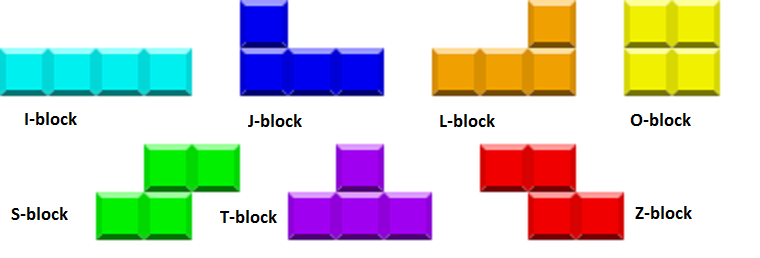
\includegraphics[scale=0.5]{resources/img/tetrominoes}
	\label{tetrominoes}
	}

\section{The position of each mino inside respective tetromino}

	\centering
	\begin{minipage}{0.2\textwidth}
		\centering
		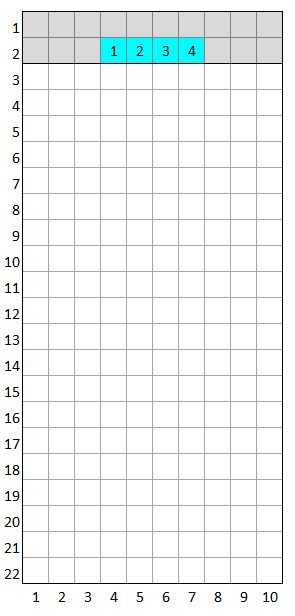
\includegraphics[scale=0.4]{resources/img/minos/mino_cyan}
		\label{fig:mino-cyan}
	\end{minipage}%
	\begin{minipage}{0.2\textwidth}
		\centering
		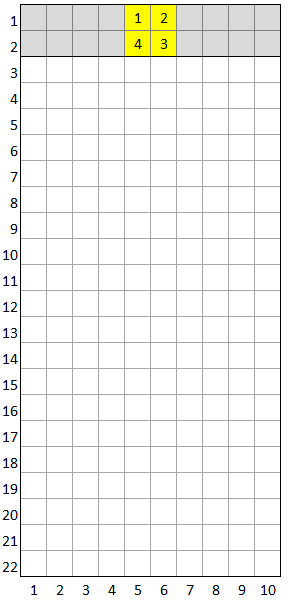
\includegraphics[scale=0.4]{resources/img/minos/mino_yellow}
		\label{fig:mino-yellow}
	\end{minipage}%
	\begin{minipage}{0.2\textwidth}
		\centering
		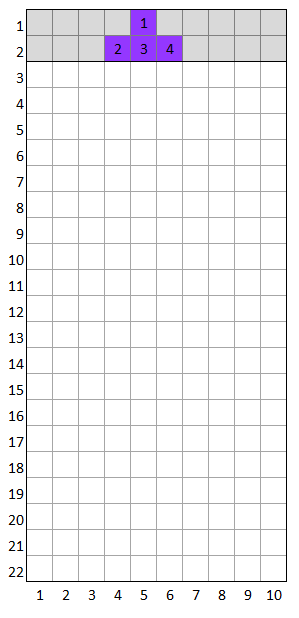
\includegraphics[scale=0.4]{resources/img/minos/mino_purple}
		\label{fig:mino-purple}
	\end{minipage}%
	\begin{minipage}{0.2\textwidth}
		\centering
		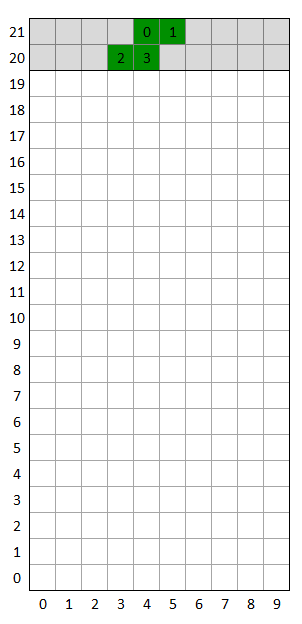
\includegraphics[scale=0.4]{resources/img/minos/mino_green}
		\label{fig:mino-green}
	\end{minipage}
	\begin{minipage}{0.26\textwidth}
		\centering
		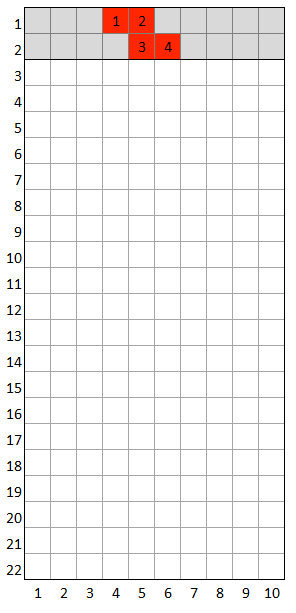
\includegraphics[scale=0.4]{resources/img/minos/mino_red}
		\label{fig:mino-red}
	\end{minipage}%
	\begin{minipage}{0.26\textwidth}
		\centering
		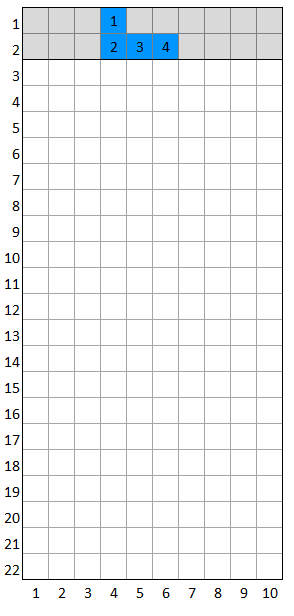
\includegraphics[scale=0.4]{resources/img/minos/mino_blue}
		\label{fig:mino-blue}
	\end{minipage}%
	\begin{minipage}{0.26\textwidth}
		\centering
		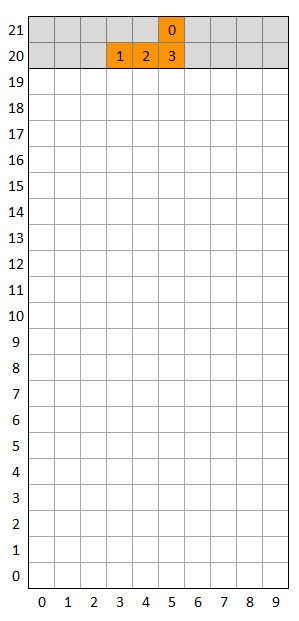
\includegraphics[scale=0.4]{resources/img/minos/mino_orange}
		\label{fig:mino-orange}
	\end{minipage}%


\section{All possible orientations of each tetromino}
	
	\begin{center}


	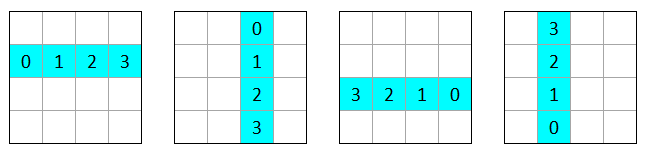
\includegraphics[scale=0.7]{resources/img/orientations/cyan}
	\label{img:cyan}

	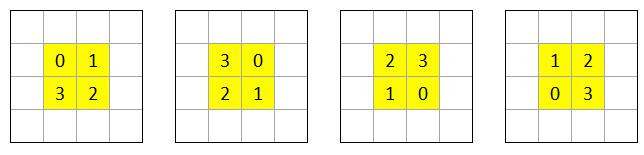
\includegraphics[scale=0.7]{resources/img/orientations/yellow}
	\label{img:yellow}

	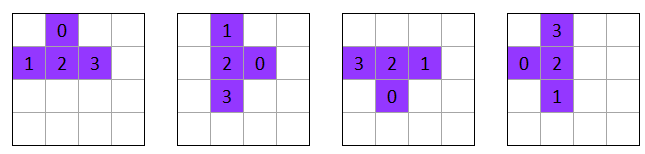
\includegraphics[scale=0.7]{resources/img/orientations/purple}
	\label{img:purple}

	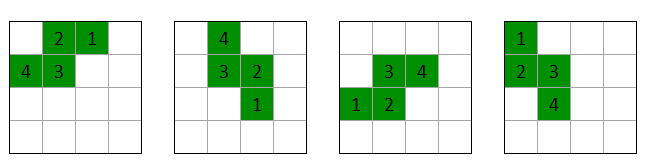
\includegraphics[scale=0.7]{resources/img/orientations/green}
	\label{img:green}

	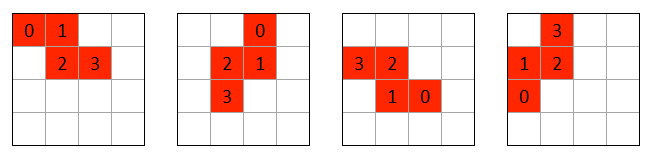
\includegraphics[scale=0.7]{resources/img/orientations/red}
	\label{img:red}

	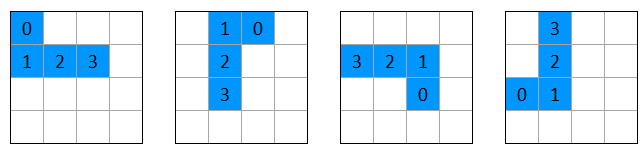
\includegraphics[scale=0.7]{resources/img/orientations/blue}
	\label{img:blue}

	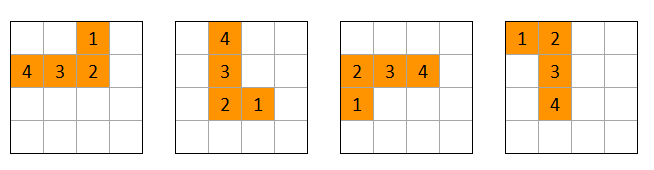
\includegraphics[scale=0.7]{resources/img/orientations/orange}
	\label{img:orange}
	
	\end{center}
	
\end{document}
